%Template_made_by_SGjTeX

\documentclass[a4paper,13pt]{book}
\usepackage[utf8]{inputenc}     
\usepackage[T1]{fontenc}
\usepackage{amsmath,amsthm, amssymb,xcolor,amsfonts,mathrsfs} 
\usepackage[left=2.5cm,right=2.5cm,top=2.5cm,bottom=2.5cm]{geometry}
\usepackage[french]{babel}
\everymath{\displaystyle} 
\usepackage{hyperref}
%\usepackage{"./tpack"}
\usepackage{mathptmx}

\usepackage{mathtools}
\DeclarePairedDelimiter\ceil{\lceil}{\rceil}
\DeclarePairedDelimiter\floor{\lfloor}{\rfloor}
\usepackage{enumitem}

\usepackage{pgfplots} % Package pour tracer les courbes
\usepackage{filecontents} % Permet d'intégrer les données dans le fichier source
\usepackage[explicit]{ titlesec}
\usepackage{fancybox}
%\usepackage{thmbox}   
%================================ 
\usepackage{fancyhdr}
\usepackage{fancybox}

\usepackage{xcolor}
\pagestyle{fancy}
\fancyhf{} 

%\fancyfoot[RO,LE]{\rightmark} 

\cfoot{\thepage}
\lfoot{}
\renewcommand{\chaptermark}[1]{\markboth{#1}{}}
%===============================
\newtheorem{definition}{Définition}[section]
\newtheorem{theo}{Théorème}[section]
\newtheorem{pro}{Proposition}[section] 
\newtheorem{cor}{Corollaire}[section]
\newtheorem{lem}{Lemme}[section]
\newtheorem{rem}{Remarque}[section]

\definecolor{gris}{gray}{0.9}
\definecolor{perfectorange}{RGB}{255,165,20}
\definecolor{darkblue}{RGB}{25,25,100}
\definecolor{darkkblue}{RGB}{0,0,50}
\definecolor{darkred}{RGB}{180,0,0}
\definecolor{green_identifiers}{RGB}{00,80,00}
\definecolor{blue_know}{RGB}{00,20,20}
\definecolor{orange_comments}{RGB}{214, 161, 126}
\definecolor{red_keywords}{RGB}{215, 103, 129}
\definecolor{black_strings}{RGB}{50, 50, 50}
%utilis� dans la partie analyse
\definecolor{fond}{rgb}{.55,.55,.92}
%fin creation couleurs
% Définir le théorème avec couleur rouge
\newtheorem{danger1}{Attention}[section]
\newenvironment{danger}{\begin{danger1}\color{darkred}}{\end{danger1}}

% Définir le théorème avec couleur verte
\newtheorem{know1}{A Savoir}[section]
\newenvironment{know}{\begin{know1}\color{blue_know}}{\end{know1}}

\renewcommand{\footrulewidth}{1pt} 
\renewcommand{\thesection}{\arabic{section}}
\renewcommand{\thesubsection}{\thesection.\arabic{subsection}}
\renewcommand{\thesubsubsection}{\thesubsection.\arabic{subsubsection}}

\newcommand{\Hrule}{
	\rule{\linewidth}{0.5mm}
}
\newcommand\justify{%
  \let\\\@centercr
  \rightskip\z@skip
  \leftskip\z@skip}
%%===exercices 
%\newcounter{ex}
\newenvironment{exe}% exple \begin{exe}...\end{exe}
{\refstepcounter{ex}%
	\par\noindent
	{\underline{\bfseries{Exercice \theex \hspace*{0.009 cm} :}} }
	\mdseries
	\slshape}
{\par
	\medskip}
%====exemples
\newcounter{exple}
\newenvironment{exple}
{\refstepcounter{exple}%
	\par\noindent
	{\underline{\bfseries{Exemple  :}} }
	\mdseries
	\slshape}
{\par
	\medskip}
%====preuve
%\newenvironment{proof}
%{\rmfamily\mdseries{\bfseries Preuve : }}
%{\hfill$\blacksquare$}
%======
\renewcommand{\baselinestretch}{1.3}  

%%%%%%%%%%%%%%%%%%%%%%%%%%%%%%%%%

\newcommand{\ps}[2]{\left\langle #1 ,#2 \right\rangle  }
%%%%%%%%%%%%%%%%%%%%%% 
\let\cleardoublepage\clearpage 

\usepackage[explicit]{titlesec}
\usepackage{minitoc}
\renewcommand{\mtctitle}{Plan}
\usepackage[most]{tcolorbox}
\newcommand\mychapter{\titleformat{\chapter}[block]{}{}{0pt}{\centering\hrule height 5pt
		\vglue-1.1 \baselineskip
		\tcbox[enhanced,colback=white,frame code={}]{\bfseries\chaptername\hskip2mm \thechapter}
		\bigskip
		\vglue-3mm\hrule \vglue3mm
		{\huge \bfseries ##1}\vglue3mm\hrule
	}[]\chapter}
\dominitoc
\usepackage{caption}
\usepackage{listings}

%%configuration de listings
\definecolor{codegreen}{rgb}{0,0.6,0}
\definecolor{codegray}{rgb}{0.5,0.5,0.5}
\definecolor{codepurple}{rgb}{0.58,0,0.82}
\definecolor{backcolour}{rgb}{0.97,0.99,0.99}

\lstdefinestyle{mystyle}{
    backgroundcolor=\color{backcolour},
    commentstyle=\color{codegreen},
    keywordstyle=\color{magenta},
    numberstyle=\tiny\color{codegray},
    stringstyle=\color{codepurple},
    basicstyle=\ttfamily\footnotesize,
    breakatwhitespace=false,
    breaklines=true,
    captionpos=b,
    keepspaces=true,
    numbers=left,
    numbersep=5pt,
    showspaces=false,
    showstringspaces=false,
    showtabs=false,
    tabsize=4
}

\lstset{style=mystyle}

\definecolor{Zgris}{rgb}{238, 238, 238}

\newsavebox{\BBbox}
\newenvironment{DDbox}[1]{
\begin{lrbox}{\BBbox}\begin{minipage}{\linewidth}}
{\end{minipage}\end{lrbox}\noindent\colorbox{Zgris}{\usebox{\BBbox}} \\
[.5cm]}
\author{\bsc{DADA SIMEU Cédric Darel}}


\begin{document}
	\graphicspath{ {../template_page_garde} }

\begin{center}
  
\includegraphics[scale=0.15]{logo.jpg}
\end{center}

{\vspace{7em}}

\begin{center}
  \begin{tabular}{|lp{5.0cm}lll|}
    \hline
    &  &  &  & {\small{2024/25}}\\
    &  &  &  & \\
    &  &  &  & \\
    \textbf{Nom:} & \bsc{DADA SIMEU Cédric Darel}
    
    \  &  &  & \\
    \textbf{Email:} & cedric-darel.dada@ensta-paris.fr
    
    \  &  &  & \\
    \textbf{Titre:} & Compte rendu TP3
    
    
    \
    
    \  &  &  & \\
    \hline
  \end{tabular}
\end{center}

\

{\vspace{7em}}

\begin{center}
  \Large{{\textbf{STIC}}}
\end{center}

{\medskip}

\begin{center}
  ENSTA Paris, Institut Polytechnique de Paris
\end{center}

{\newpage}

\tableofcontents
\listoffigures
\newpage
\section{Architecture matérielle de l'ordinateur}
\begin{figure}[!h]
  \begin{center}
  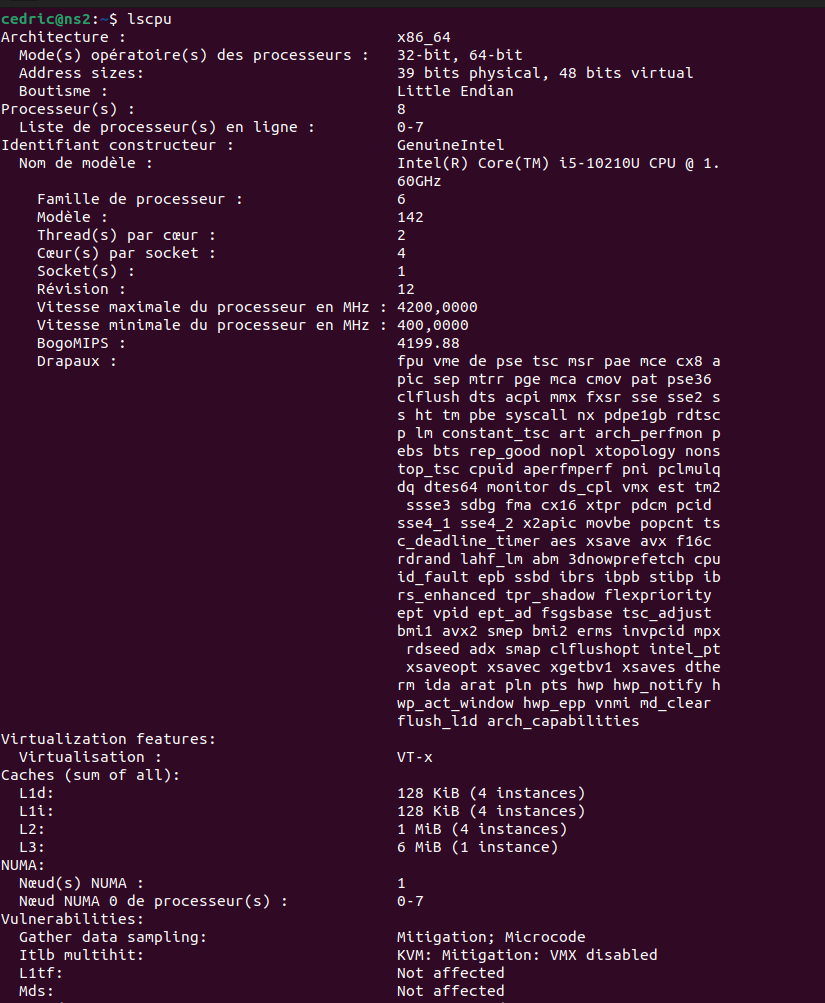
\includegraphics[scale=0.5]{../images/lscpu.png}
  \caption{Résultat de la commande lscpu}
  \label{fig:lscpu}
\end{center}
\end{figure}


\begin{figure}[!h]
  \begin{center}
      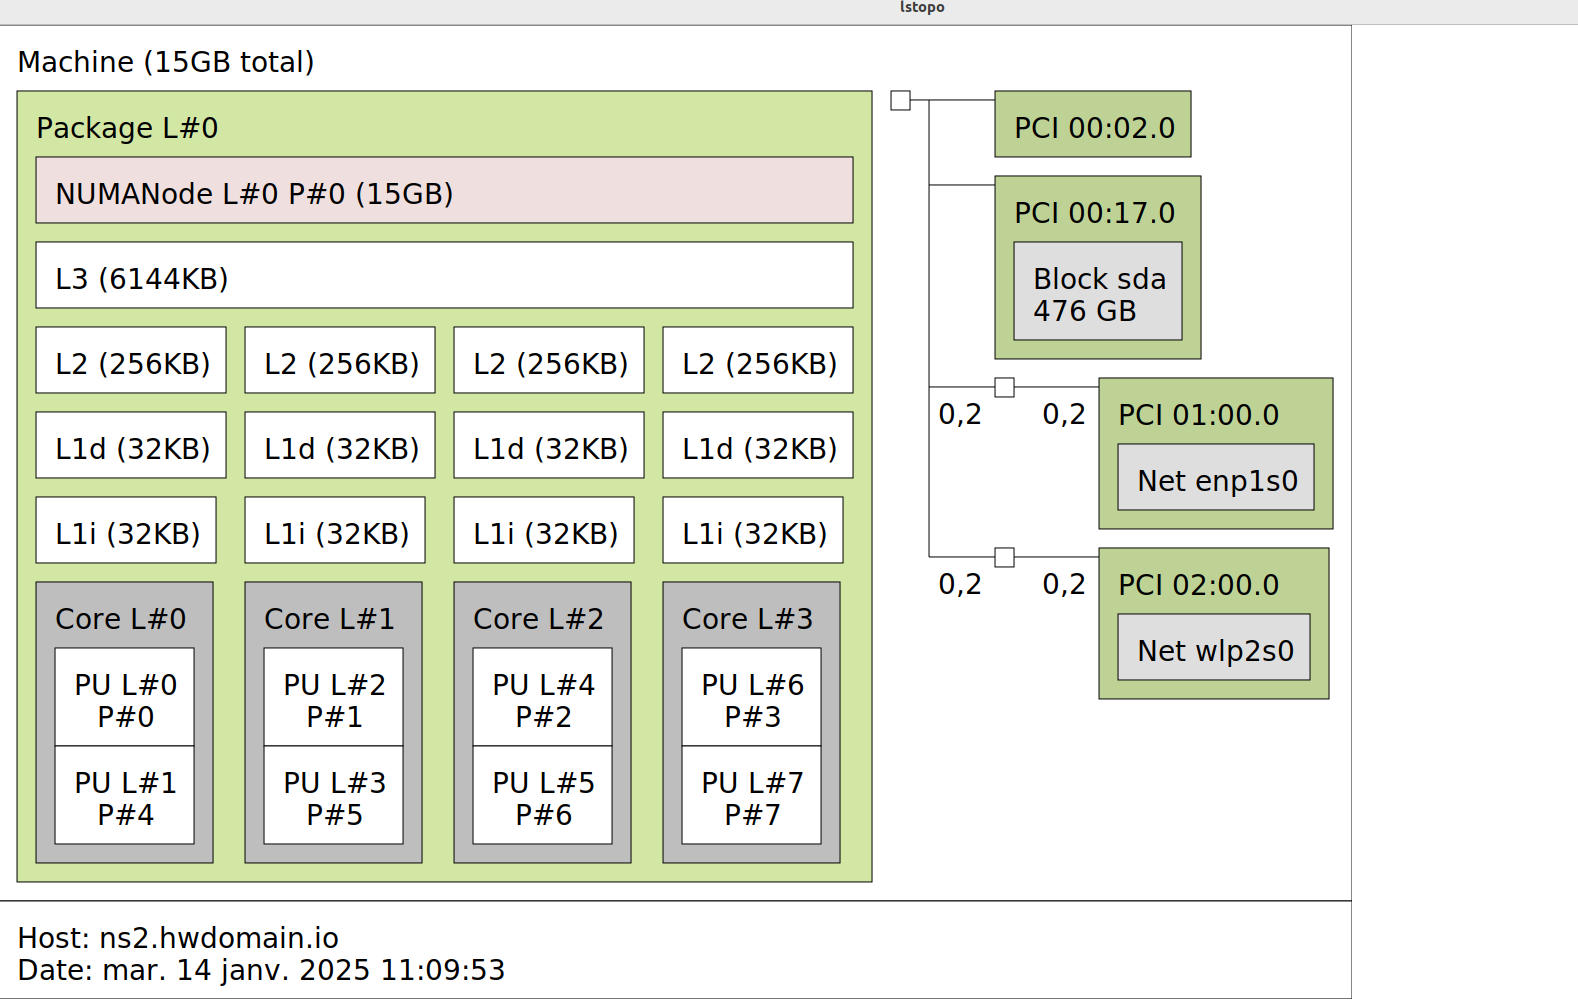
\includegraphics[scale=0.3]{../images/lstopo.png}
      \caption{Résultat de la commande lstopo : Nous pouvons visualiser les tailles des caches}
      \label{tab:ls_topo}
  \end{center}
\end{figure}
\clearpage
\section{Présentation de l'algorithme et choix des intervalles dans les buckets}
\subsection{Génération des données}

\begin{itemize}
  \item Le processus 0 génère un tableau de nombres aléatoires.
  \item La génération est faite avec np.random.rand(N) où N est le nombre total d'éléments à trier
  \item np.random.seed(42), nous garantit que nos différents tests seront réalisés avec les memes valeurs de la liste, ce qui rend les interprétations possibles.
\end{itemize}
\subsection{Distribution des données}
Les données sont distribuées entre les processus via Scatterv. Chaque processus reçoit une portion égale ou presque égale des données.
\subsection{Tri local}
Chaque processus trie localement sa portion de données avec local\_data.sort(), sachant que la méthode sort utilise le tri rapide par défaut.
\subsection{Détermination des intervalles(bornes) des buckets}
 \begin{itemize}
  \item Chaque processus sélectionne des échantillons régulièrement espacés dans ses données locales.
  \item Ces échantillons sont rassemblés sur le processus 0 avec comm.gather
  \item Sur le processus 0, les échantillons sont triés, et des bornes sont définies en divisant l'espace des valeurs en segments égaux.
  \item Les bornes sont ensuite diffusées à tous les processus avec comm.bcast.
 \end{itemize}
 \subsection{Redistribution des données}
 Les données sont redistribuées selon les bornes des buckets :
 \begin{itemize}
  \item Chaque processus détermine combien d'éléments il doit envoyer à chaque autre processus.
  \item Les données sont redistribuées avec Alltoallv.
 \end{itemize}
 \subsection{Tri final et collecte}
 \begin{itemize}
  \item Après redistribution, chaque processus trie localement ses nouvelles données.
  \item Les résultats sont rassemblés sur le processus 0 avec comm.gather.
 \end{itemize}

\section{Analyse de la complexité}
D'après le cours, la complexité du bucket sort parrallèle est donnée par :
\[
  T_{\text{total}} = O(N + \frac{N}{k} log_2 (\frac{N}{k}))
\]
Où k = n (nombre de buckets = nombre de processus).

Pour une distribution équilibrée des données: 
\begin{itemize}
  \item Le cout local de tri est $O(\frac{N}{n}log_2 (\frac{N}{n}))$
  \item Le cout de redistribution est proportionnel à $O(\frac{N}{n})$
\end{itemize}
\section{Expérimentation et Résultats}
\begin{know}
Les données ayant permi la réalisation des différents graphes et tableaux qui suivent sont disponibles dans le fichier tests.txt
\end{know}
\begin{itemize}
    \item Le tableau \ref{tab:execution_time_total} résume le temps total d'exécution pour chaque combinaison de N(taille du tableau à trier) et n(nombre de processus).
    \item Dans, le tableau \ref{tab:speedup} le speedup est calculé comme étant : $S(n) = \frac{T(2)}{T(n)}$
    \item Dans le tableau, \ref{tab:efficiency}, $E(n)=\frac{S(n)}{n}$
    \item Le graphique \ref{fig:execution_time_vs_n} montre le temps d'exécution total pour chaque valeur de N en fonction du nombre de processus.
    \item Le graphique \ref{fig:efficiency_vs_n} montre l'efficiency pour chaque valeur de N en fonction du nombre de processus.
    \item Le graphique \ref{fig:speedup_vs_n} montre le speedup pour chaque valeur de N en fonction du nombre de processus.
    \item Le graphique \ref{fig:load_imbalance_vs_n} présente le déséquilibrage des charges pour chaque valeur de N en fonction du nombre de processus.\\
    Ce déséquilibrage est donné par la formule $\text{Déséquilibrage (\%)} = \frac{\text{max(local\_sort)} - \text{min(local\_sort)}}{\text{max(local\_sort)}} \times 100$
\end{itemize}
\begin{table}[ht]
  \centering
  \caption{Temps d'exécution total pour différentes valeurs de $ N $ et $ n $.}
  \label{tab:execution_time_total}
  \begin{tabular}{@{}ccccccc@{}}
    \toprule
    $ N $ & $ n = 2 $ & $ n = 3 $ & $ n = 4 $ & $ n = 8 $ & $ n = 16 $ \\
    \midrule
    $ 10^3 $ & 0.007857 & 0.008237 & 0.091724 & 0.017107 & 0.294403 \\
    $ 10^4 $ & 0.015728 & 0.016078 & 0.085148 & 0.034283 & 0.525791 \\
    $ 10^5 $ & 0.094280 & 0.084637 & 0.216848 & 0.159568 & 1.188889 \\
    $ 10^6 $ & 0.965147 & 0.715270 & 0.878063 & 0.688540 & 1.198288 \\
    $ 10^7 $ & 10.276568 & 6.984677 & 8.705777 & 6.583885 & 13.667255 \\
    $ 10^8 $ & 10.181517 & 7.492297 & 9.834438 & 8.913589 & 22.307478 \\
    \bottomrule
  \end{tabular}
\end{table}
\begin{table}[ht]
  \centering
  \caption{Déséquilibrage des charges en fonction de $ N $ et $ n $.}
  \label{tab:load_imbalance}
  \begin{tabular}{@{}cccccc@{}}
    \toprule
    $ N $ & $ n = 2 $ & $ n = 3 $ & $ n = 4 $ & $ n = 8 $ & $ n = 16 $ \\
    \midrule
    $ 10^3 $ & 11.11\% & 15.79\% & 15.38\% & 38.46\% & 77.78\% \\
    $ 10^4 $ & 10.00\% & 17.65\% & 20.00\% & 38.46\% & 77.78\% \\
    $ 10^5 $ & 1.79\% & 17.65\% & 15.38\% & 25.00\% & 40.00\% \\
    $ 10^6 $ & 1.49\% & 11.76\% & 15.38\% & 25.00\% & 40.00\% \\
    $ 10^7 $ & 1.49\% & 11.76\% & 15.38\% & 25.00\% & 40.00\% \\
    $ 10^8 $ & 1.79\% & 17.65\% & 15.38\% & 25.00\% & 40.00\% \\
    \bottomrule
  \end{tabular}
\end{table}
\begin{table}[ht]
  \centering
  \caption{Speedup pour différentes valeurs de $ N $ et $ n $.}
  \label{tab:speedup}
  \begin{tabular}{@{}ccccccc@{}}
    \toprule
    $ N $ & $ n = 2 $ & $ n = 3 $ & $ n = 4 $ & $ n = 8 $ & $ n = 16 $ \\
    \midrule
    $ 10^3 $ & 1.00 & 0.95 & 0.09 & 0.57 & 0.03 \\
    $ 10^4 $ & 1.00 & 0.98 & 0.18 & 0.46 & 0.03 \\
    $ 10^5 $ & 1.00 & 1.11 & 0.44 & 0.60 & 0.08 \\
    $ 10^6 $ & 1.00 & 1.48 & 1.10 & 1.40 & 0.81 \\
    $ 10^7 $ & 1.00 & 1.47 & 1.18 & 1.56 & 0.75 \\
    $ 10^8 $ & 1.00 & 1.36 & 1.04 & 1.15 & 0.45 \\
    \bottomrule
  \end{tabular}
\end{table}

\begin{table}[ht]
  \centering
  \caption{Efficiency pour différentes valeurs de $ N $ et $ n $.}
  \label{tab:efficiency}
  \begin{tabular}{@{}ccccccc@{}}
    \toprule
    $ N $ & $ n = 2 $ & $ n = 3 $ & $ n = 4 $ & $ n = 8 $ & $ n = 16 $ \\
    \midrule
    $ 10^3 $ & 0.50 & 0.32 & 0.02 & 0.07 & 0.00 \\
    $ 10^4 $ & 0.50 & 0.33 & 0.05 & 0.06 & 0.00 \\
    $ 10^5 $ & 0.50 & 0.37 & 0.11 & 0.08 & 0.01 \\
    $ 10^6 $ & 0.50 & 0.49 & 0.28 & 0.18 & 0.05 \\
    $ 10^7 $ & 0.50 & 0.49 & 0.29 & 0.20 & 0.05 \\
    $ 10^8 $ & 0.50 & 0.45 & 0.26 & 0.14 & 0.03 \\
    \bottomrule
  \end{tabular}
\end{table}


\begin{figure}[ht]
  \centering
  \begin{tikzpicture}
    \begin{axis}[
      xlabel={Nombre de Processus ($ n $)},
      ylabel={Temps d'exécution (s)},
      legend pos=north west,
      width=12cm,
      height=9cm 
      ]
      % N = 10^3
      \addplot coordinates {
        (2, 0.007857)
        (3, 0.008237)
        (4, 0.091724)
        (8, 0.017107)
        (16, 0.294403)
      };
      \addlegendentry{$ N = 10^3 $};
      
      % N = 10^4
      \addplot coordinates {
        (2, 0.015728)
        (3, 0.016078)
        (4, 0.085148)
        (8, 0.034283)
        (16, 0.525791)
      };
      \addlegendentry{$ N = 10^4 $};
      
      % N = 10^5
      \addplot coordinates {
        (2, 0.094280)
        (3, 0.084637)
        (4, 0.216848)
        (8, 0.159568)
        (16, 1.188889)
      };
      \addlegendentry{$ N = 10^5 $};
      
      % N = 10^6
      \addplot coordinates {
        (2, 0.965147)
        (3, 0.715270)
        (4, 0.878063)
        (8, 0.688540)
        (16, 1.198288)
      };
      \addlegendentry{$ N = 10^6 $};
      
      % N = 10^7
      \addplot coordinates {
        (2, 10.276568)
        (3, 6.984677)
        (4, 8.705777)
        (8, 6.583885)
        (16, 13.667255)
      };
      \addlegendentry{$ N = 10^7 $};
      
      % N = 10^8
      \addplot coordinates {
        (2, 10.181517)
        (3, 7.492297)
        (4, 9.834438)
        (8, 8.913589)
        (16, 22.307478)
      };
      \addlegendentry{$ N = 10^8 $};
    \end{axis}
  \end{tikzpicture}
  \caption{Temps d'exécution vs nombre de processus.}
  \label{fig:execution_time_vs_n}
\end{figure}
\begin{figure}[ht]
  \centering
  \begin{tikzpicture}
    \begin{axis}[
      xlabel={Nombre de Processus ($ n $)},
      ylabel={Déséquilibrage des Charges (\%)},
      legend pos=north west,
      width=12cm,
      height=9cm,
      tick label style={font=\large}, % Augmente la taille des étiquettes des ticks
      legend cell align=left,         % Aligne les entrées de la légende à gauche
      ]
      % N = 10^3
      \addplot[color=blue, mark=*, line width=1.5pt] coordinates {
        (2, 11.11)
        (3, 15.79)
        (4, 15.38)
        (8, 38.46)
        (16, 77.78)
      };
      \addlegendentry{$ N = 10^3 $};
      
      % N = 10^4
      \addplot[color=red, mark=square*, line width=1.5pt] coordinates {
        (2, 10.00)
        (3, 17.65)
        (4, 20.00)
        (8, 38.46)
        (16, 77.78)
      };
      \addlegendentry{$ N = 10^4 $};
      
      % N = 10^5
      \addplot[color=green, mark=triangle*, line width=1.5pt] coordinates {
        (2, 1.79)
        (3, 17.65)
        (4, 15.38)
        (8, 25.00)
        (16, 40.00)
      };
      \addlegendentry{$ N = 10^5 $};
      
      % N = 10^6
      \addplot[color=orange, mark=diamond*, line width=1.5pt] coordinates {
        (2, 1.49)
        (3, 11.76)
        (4, 15.38)
        (8, 25.00)
        (16, 40.00)
      };
      \addlegendentry{$ N = 10^6 $};
      
      % N = 10^7
      \addplot[color=purple, mark=x, line width=1.5pt] coordinates {
        (2, 1.49)
        (3, 11.76)
        (4, 15.38)
        (8, 25.00)
        (16, 40.00)
      };
      \addlegendentry{$ N = 10^7 $};
      
      % N = 10^8
      \addplot[color=brown, mark=+, line width=1.5pt] coordinates {
        (2, 1.79)
        (3, 17.65)
        (4, 15.38)
        (8, 25.00)
        (16, 40.00)
      };
      \addlegendentry{$ N = 10^8 $};
    \end{axis}
  \end{tikzpicture}
  \caption{Déséquilibrage des charges vs nombre de processus.}
  \label{fig:load_imbalance_vs_n}
\end{figure}
\begin{figure}[ht]
  \centering
  \begin{tikzpicture}
    \begin{axis}[
      xlabel={Nombre de Processus ($ n $)},
      ylabel={Temps (secondes)},
      legend pos=north west, % Légende en bas à droite
      width=12cm,
      height=9cm,
      tick label style={font=\large}, % Augmente la taille des étiquettes des ticks
      ]
      % Temps de communication (scatter + redistribute + gather)
      \addplot[color=blue, mark=*, line width=1.5pt] coordinates {
        (2, 0.000431)
        (3, 0.000697)
        (4, 0.011921)
        (8, 0.029807)
        (16, 0.076764)
      };
      \addlegendentry{Temps de communication};
      
      % Temps de calcul local (local_sort)
      \addplot[color=red, mark=square*, line width=1.5pt] coordinates {
        (2, 0.000036)
        (3, 0.000247)
        (4, 0.022649)
        (8, 0.145621)
        (16, 2.120518)
      };
      \addlegendentry{Temps de calcul local};
    \end{axis}
  \end{tikzpicture}
  \caption{Comparaison entre temps de communication et temps de calcul local pour $ N = 10^6 $.}
  \label{fig:comm_vs_comp}
\end{figure}
\begin{figure}[ht]
  \centering
  \begin{tikzpicture}
    \begin{axis}[
      xlabel={Nombre de Processus ($ n $)},
      ylabel={Speedup},
      legend pos=north east,
      width=13cm,
      height=11cm,
      tick label style={font=\large}, % Augmente la taille des étiquettes des ticks
      ]
      % N = 10^3
      \addplot coordinates {
        (2, 1.00)
        (3, 0.95)
        (4, 0.09)
        (8, 0.57)
        (16, 0.03)
      };
      \addlegendentry{$ N = 10^3 $};
      
      % N = 10^4
      \addplot coordinates {
        (2, 1.00)
        (3, 0.98)
        (4, 0.18)
        (8, 0.46)
        (16, 0.03)
      };
      \addlegendentry{$ N = 10^4 $};
      
      % N = 10^5
      \addplot coordinates {
        (2, 1.00)
        (3, 1.11)
        (4, 0.44)
        (8, 0.60)
        (16, 0.08)
      };
      \addlegendentry{$ N = 10^5 $};
      
      % N = 10^6
      \addplot coordinates {
        (2, 1.00)
        (3, 1.48)
        (4, 1.10)
        (8, 1.40)
        (16, 0.81)
      };
      \addlegendentry{$ N = 10^6 $};
      
      % N = 10^7
      \addplot coordinates {
        (2, 1.00)
        (3, 1.47)
        (4, 1.18)
        (8, 1.56)
        (16, 0.75)
      };
      \addlegendentry{$ N = 10^7 $};
      
      % N = 10^8
      \addplot coordinates {
        (2, 1.00)
        (3, 1.36)
        (4, 1.04)
        (8, 1.15)
        (16, 0.45)
      };
      \addlegendentry{$ N = 10^8 $};
    \end{axis}
  \end{tikzpicture}
  \caption{Speedup vs nombre de processus.}
  \label{fig:speedup_vs_n}
\end{figure}
\begin{figure}[ht]
  \centering
  \begin{tikzpicture}
    \begin{axis}[
      xlabel={Nombre de Processus ($ n $)},
      ylabel={Efficiency (\% )},
      legend pos=north east,
      width=13cm,
      height=10cm,
      tick label style={font=\large}, % Augmente la taille des étiquettes des ticks
      ]
      % N = 10^3
      \addplot coordinates {
        (2, 0.50)
        (3, 0.32)
        (4, 0.02)
        (8, 0.07)
        (16, 0.00)
      };
      \addlegendentry{$ N = 10^3 $};
      
      % N = 10^4
      \addplot coordinates {
        (2, 0.50)
        (3, 0.33)
        (4, 0.05)
        (8, 0.06)
        (16, 0.00)
      };
      \addlegendentry{$ N = 10^4 $};
      
      % N = 10^5
      \addplot coordinates {
        (2, 0.50)
        (3, 0.37)
        (4, 0.11)
        (8, 0.08)
        (16, 0.01)
      };
      \addlegendentry{$ N = 10^5 $};
      
      % N = 10^6
      \addplot coordinates {
        (2, 0.50)
        (3, 0.49)
        (4, 0.28)
        (8, 0.18)
        (16, 0.05)
      };
      \addlegendentry{$ N = 10^6 $};
      
      % N = 10^7
      \addplot coordinates {
        (2, 0.50)
        (3, 0.49)
        (4, 0.29)
        (8, 0.20)
        (16, 0.05)
      };
      \addlegendentry{$ N = 10^7 $};
      
      % N = 10^8
      \addplot coordinates {
        (2, 0.50)
        (3, 0.45)
        (4, 0.26)
        (8, 0.14)
        (16, 0.03)
      };
      \addlegendentry{$ N = 10^8 $};
    \end{axis}
  \end{tikzpicture}
  \caption{Efficiency vs nombre de processus.}
  \label{fig:efficiency_vs_n}
\end{figure}

\clearpage
\subsection{Configuration matérielle }
Le mode d'exécution --oversubscribe était nécesaire pour exécuter plus de 4 processus MPI sur notre machine qui ne contient que 4 coeurs physiques. (voir fig \ref{fig:lscpu}).
\subsubsection{Impact de l'oversubscription}  L'oversubscription signifie que plusieurs processus partagent le même cœur physique, ce qui peut entraîner :
\begin{itemize}
  \item Contestation des ressources  : Les processus doivent partager les caches et les unités de calcul, augmentant potentiellement les délais d'accès mémoire et réduisant les performances.
  \item Overhead du multitâche  : Le système d'exploitation doit constamment basculer entre les threads, introduisant un coût supplémentaire lié au context-switching.
\end{itemize} 

\subsection{Analyse  et interprétation des résultats}
\subsubsection{Temps d'exécution total} Le temps total d'exécution augmente lorsque n>4, surtout pour de grandes valeurs de N. Cela est dû à : 
\begin{itemize}
  \item Communication accrue : Plus il y a de processus, plus les communications inter-processus (scatter, redistribute, gather) deviennent coûteuses.
  \item Oversubscription  : Au-delà de 4 processus, les threads partagent les mêmes cœurs physiques, réduisant l'efficacité du parallélisme.
\end{itemize}
\subsubsection{Speedup et Efficiency}
\begin{itemize}
  \item Pour $N<10^5$, le speedup diminue rapidement lorsque n>4, car les communications dominent les calculs locaux.
  \item Pour $N\geq 10^6$, le speedup reste raisonnable jusqu'à n=8, mais chute pour n=16 en raison de l'oversubscription et des communications excessives.
  \item L'efficiency chute significativement pour n>8, indiquant un mauvais équilibre entre les calculs et les communications.
  \item Pour $N\geq 10^6$, le déséquilibrage reste modéré jusqu'à n=4, mais augmente pour n>4, en partie à cause de l'oversubscription.
\end{itemize}
\subsubsection{Impact des surcouts de communication}
Les phases de communication (scatter, redistribute, gather) représentent une part importante du temps total d'exécution, surtout pour n>4.
\begin{itemize}
  \item Pour $N=10^3$ ou $10^4$, \textbf{les communications dominent les calculs locaux}, rendant l'utilisation de nombreux processus inefficace.
  \item Pour $N\geq 10^6$, les communications restent importantes, mais leur impact relativement aux temps de calcul diminue à mesure que N augmente, car les calculs locaux (local\_sort) deviennent plus coûteux.
\end{itemize}

\end{document}
